\apendice{Plan de Proyecto Software}

\section{Introducción}
Siendo el presente un proyecto destinado al desarrollo del backend para una aplicación móvil que pretende colaborar a la mejora de la calidad de vida de un colectivo, en este caso las personas con Esclerosis Múltiple (en adelante EM), es necesario incluir información relevante. La misma refereria a su planificación, viabilidad y costos, que permita tener una visión panorámica completa y exhaustiva de todas las implicaciones del proyecto, junto con su evolución y la forma en que se llevó a cabo; a saber:

\section{Planificación temporal}
Para el desarrollo del presente proyecto se aplicó la metodología \emph{Scrum}, que es un enfoque ágil para la gestión de proyectos que se utiliza comúnmente en el desarrollo de software y otros proyectos complejos. Se enfoca en equipos pequeños, autoorganizados y multifuncionales que trabajan juntos para lograr metas específicas en ciclos cortos llamados sprints, aplicando la estrategia de desarrollo incremental. \\
No obstante, es importante destacar el hecho de que, si bien en Scrum se trabaja en equipos de entre 4 a 8 personas, en este caso se trabajó de forma individual por tratarse de un proyecto educativo desarrollado por un único participante. En este sentido, se siguieron los siguientes pasos:\\

\begin{itemize}
\tightlist
\item
    Cada semana se realizaron sprints cuyo propósito fue avanzar en las unidades de trabajo del proyecto y las entregas incrementales.
\item
    Al comienzo de cada sprint, en la planificación, se definieron los objetivos y tareas específicas que se debían completar.
\item 
    Las tareas se estimaron y priorizaron en función del valor que cada una aportaba al cumplimiento de los objetivos definidos, y de su complejidad; esto en un tablero backlog. 
\item 
    Durante cada sprint se llevaron a cabo las tareas establecidas en la planificación, exceptuando los \emph{bugs}.
\item 
    En el caso de que al finalizar el sprint y se completara una funcionalidad se liberaba mediante un \emph{release}. 
\item 
    Se efectuó la revisión de cada sprint para analizar el trabajo completado y generar feedback para mejorar el proyecto.
\item
    El progreso del proyecto se monitorizó mediante gráficos de \emph{burndown}, \emph{velocity} y \emph{burnup}.
\item 
    Se implementó Kanban dividido en 3 columnas, \emph{To Do}, \emph{In Progress} y \emph{Done}, para la gestión del estado de las tarjetas durante el progreso del desarrollo.
\item 
    Para el seguimiento de las tareas se utilizó la herramienta \emph{JIRA}.
    
\end{itemize}
Es importante mencionar que la estimación de tiempo destinado para cada tarea se efectuó mediante \emph{story points} basados en la serie de fibonacci, que a su vez se basaron en el grado de complejidad de cada tarea y no el número de horas que tomaría cada una.

\subsection{Sprint 0 (12/01/23 - 19/01/23)}\label{sprint-0-120123---190123}
El sprint 0 fue el kick off inicial para establecer la primera reunión con el tutor y delinear los objetivos que tendríamos durante el desarrollo del TFG.
Durante esa semana se trabajó en analizar el proyecto y su viabilidad de llevarlo a cabo, debido a los acotados plazos con los que se contaba, y al ser un desarrollo del cual se debería indigar la forma en que se podrían realizar las pruebas al finalizar el desarrollo por parte del tribunal de la Universidad.

\subsection{Sprint 1 (19/01/23 - 26/01/23)}\label{sprint-0-190123---260123}
Se realizó una investigación de mercado para poder entender qué aplicaciones existían actualmente y qué necesidades cubrían para los personas afectadas con EM. En este análisis se consideraron las aplicaciones Cleo, ME, Control EM y Emylin, y en base a ello se elaboró una propuesta de cómo se representarían y manejarían los datos dentro de la aplicación y qué funcionalidades y operaciones podría tener la misma de cara a los usuarios.

\subsection{Sprint 2 (26/01/23 - 02/02/23)}\label{sprint-0-190123---020223}
Luego de llevado a cabo el análisis del sprint 1, se solicitó una reunión con la Asociación EMUR (única organización de la sociedad civil abocada a la EM), que se coordinó para la semana siguiente al presente sprint. Durante el transcurso de esta semana se trabajó en realizar la presentación en formato Power Point para mostrar a EMUR la estructura de datos realizada.

\subsection{Sprint 3 (09/02/23 - 16/02/23)}\label{sprint-0-090223---160223}
En este sprint se llevó a cabo la reunión con la Organización, donde se mostró la  \href{https://www.dropbox.com/scl/fi/w0ks6nw8b2dslr4br24gp/TFG-Presentacion-EMUR.pptx?dl=0&rlkey=p7cyihykf6o1vnc2bfdkuhael}{presentación confeccionada}, se explicitó cómo se estructurarían los datos para poder validar las funcionalidades pensadas durante la fase previa y cómo éstos serían guardados.
De esta reunión se desprendieron algunas modificaciones mínimas respecto a la estructura de datos, principalmente en cuanto a agregar un registro médico de la persona donde la Asociación pudiera conocer qué otras comorbilidades tiene cada paciente entre otras características.

\subsection{Sprint 4 (16/02/23 - 23/02/23)}\label{sprint-0-090223---23022023}
Se comienza a hacer el diagrama de la base de datos en la herramienta \href{https://drive.google.com/file/d/1h34iN2JwS4Tcr9MRbupvjsVVfN3LC1cf/view?usp=sharing}{draw.io} basado en la estructura de datos que se aprobó por parte de la comisión directiva de EMUR. Es de mencionar que el trabajo comenzó primero por crear la tabla referente a usuarios.

\subsection{Sprint 5 (16/02/23 - 23/02/23)}\label{sprint-0-090223---230223}
Durante este sprint se creó la estructura del proyecto y la organización de carpetas basándonos en que íbamos a trabajar con una arquitectura hexagonal; como parte del mismo proceso se creó el repositorio en Github.

\subsection{Sprint 6 (23/02/23 - 02/03/23)}\label{sprint-0-090223---02032023}
En el sprint 6 se comienza a trabajar en el proyecto utilizando las metodología ágil de \emph{Scrum} con la herramienta \emph{Jira}.
Durante esta fase se desarrolló las migraciones de la base de datos y se probó su ejecución, tal como se puede ver en el \href{https://bullquine.atlassian.net/jira/software/projects/EMUR/boards/1/reports/burndown?source=overview}{siguiente enlace.}\\
Favor apreciar el gráfico de burndown chart referente a ejecución de las tareas en este sprint, (ver figura~\ref{Img:Sprint+6}).


\begin{figure}[h]
    \centering
    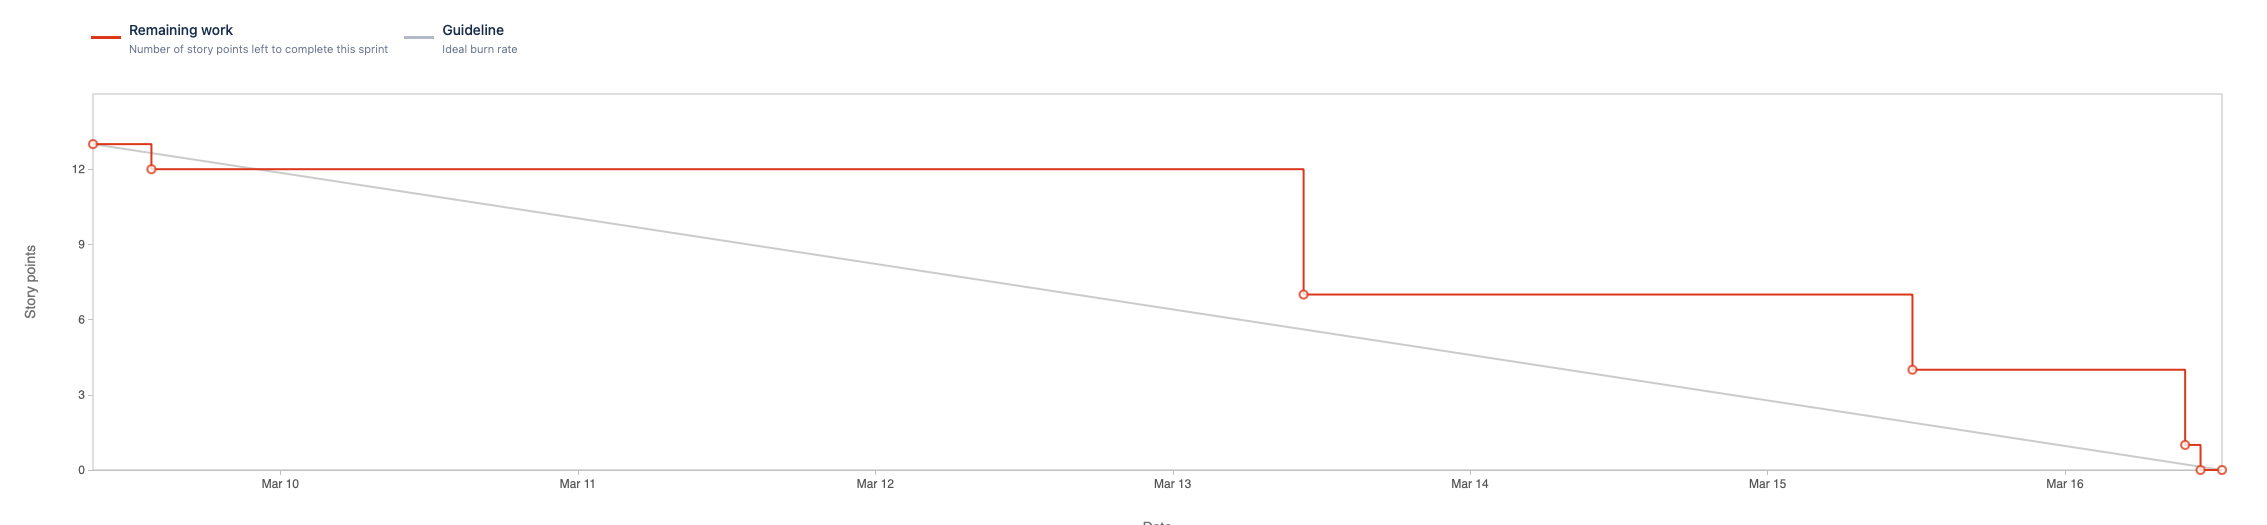
\includegraphics[width=1.0\textwidth]{img/sprint/sprint6.png}
    \caption{Sprint 6} \label{Img:Sprint+6}
\end{figure} 

\subsection{Sprint 7 (09/03/23 - 16/03/23)}\label{sprint-0-090223---160323}
Durante este sprint se comenzó a trabajar en el desarrollo de los endpoints para crear, editar, eliminar y actualizar los datos del usuario. Asimismo, se agregó el requisito de que los usuarios administradores puedan dar de baja un usuario o no permitir algún ingreso debido a actitud sospechosa.\\
Favor apreciar el gráfico de burndown chart referente a ejecución de las tareas en este sprint, (ver figura~\ref{Img:Sprint+7}).

\begin{figure}[h]
    \centering
    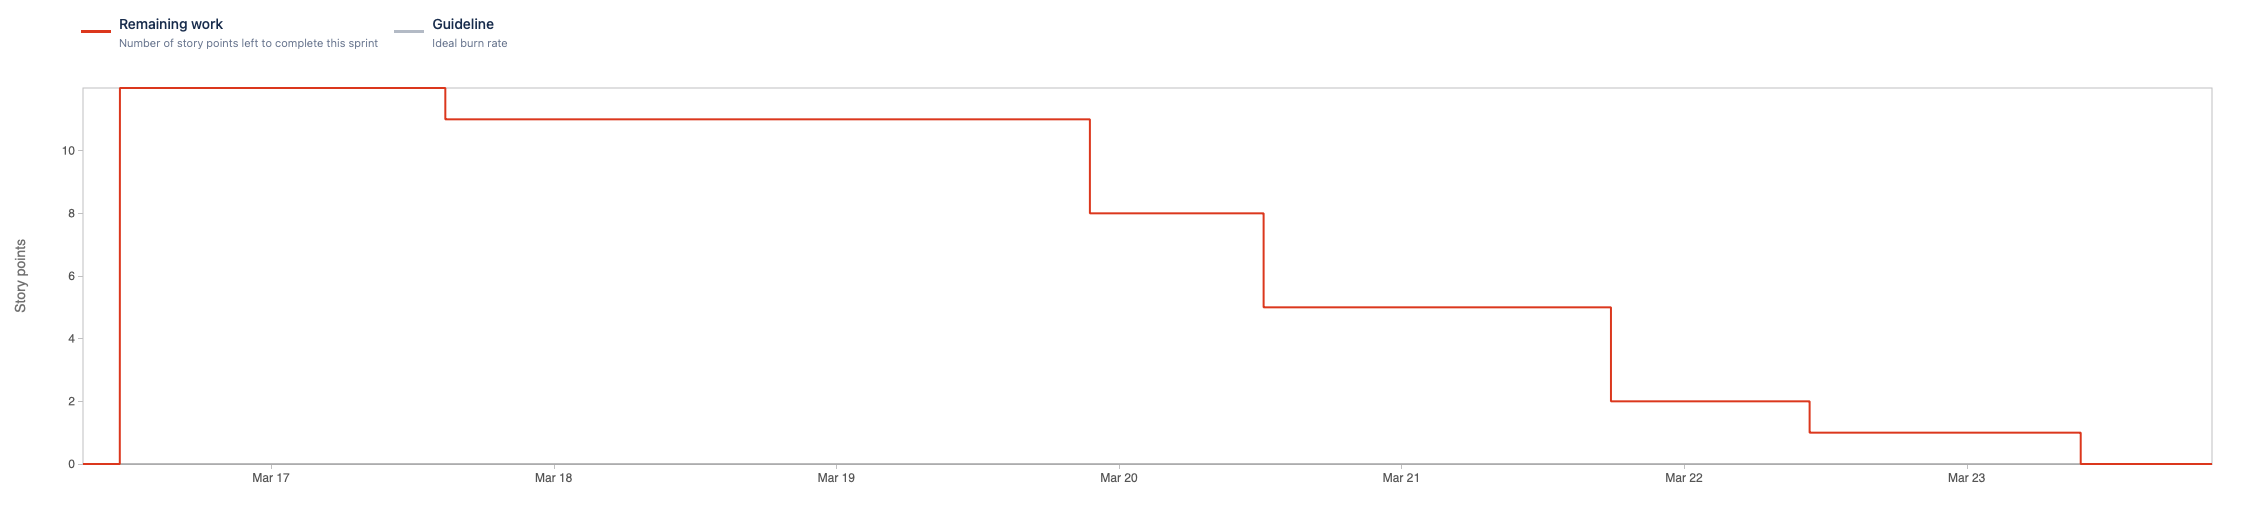
\includegraphics[width=1.0\textwidth]{img/sprint/sprint7.png}
    \caption{Sprint 7} \label{Img:Sprint+7}
\end{figure} 

\subsection{Sprint 8 (23/03/23 - 30/03/23)}\label{sprint-0-230323---300323}
En este sprint se trabajó para agregar la capa de seguridad a los endpoints, mediante el uso de JWT (JSON Web Token), así como también se crearon los test unitarios. El trabajo no fue completado en la fecha pactada debido a inconvenientes en cuanto a conocimiento sobre la validación del token JWT en el middleware de la API.\\
Favor apreciar el gráfico de burndown chart referente a ejecución de las tareas en este sprint, (ver figura~\ref{Img:Sprint+8}).

\begin{figure}[h]
    \centering
    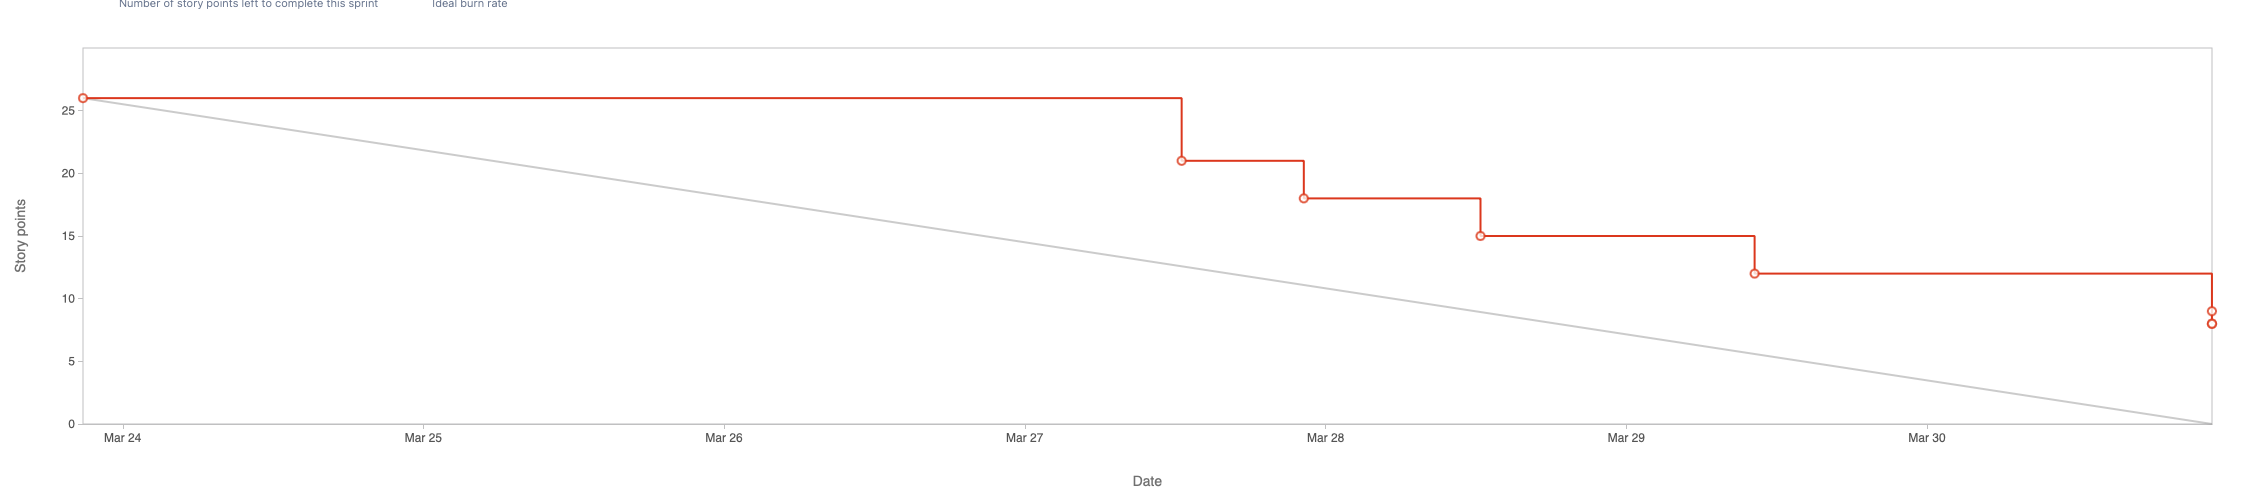
\includegraphics[width=1.0\textwidth]{img/sprint/sprint8.png}
    \caption{Sprint 8} \label{Img:Sprint+8}
\end{figure} 

\subsection{Sprint 9 (31/03/23 - 07/04/23)}\label{sprint-0-310323---070423}
Durante este sprint se pudo desbloquear el trabajo con JWT y se avanzó en la creación de los endpoints para los artículos. Asimismo, se modificó la forma de trabajar respecto a generar tipos de endpoints según características, como por ejemplo para deporte, ocio, recetas, etc, ello se resolvió utilizando el tipo artículos con un filtro por categorías.\\
Favor apreciar el gráfico de burndown chart referente a ejecución de las tareas en este sprint, (ver figura~\ref{Img:Sprint+9}).
\begin{figure}[h]
    \centering
    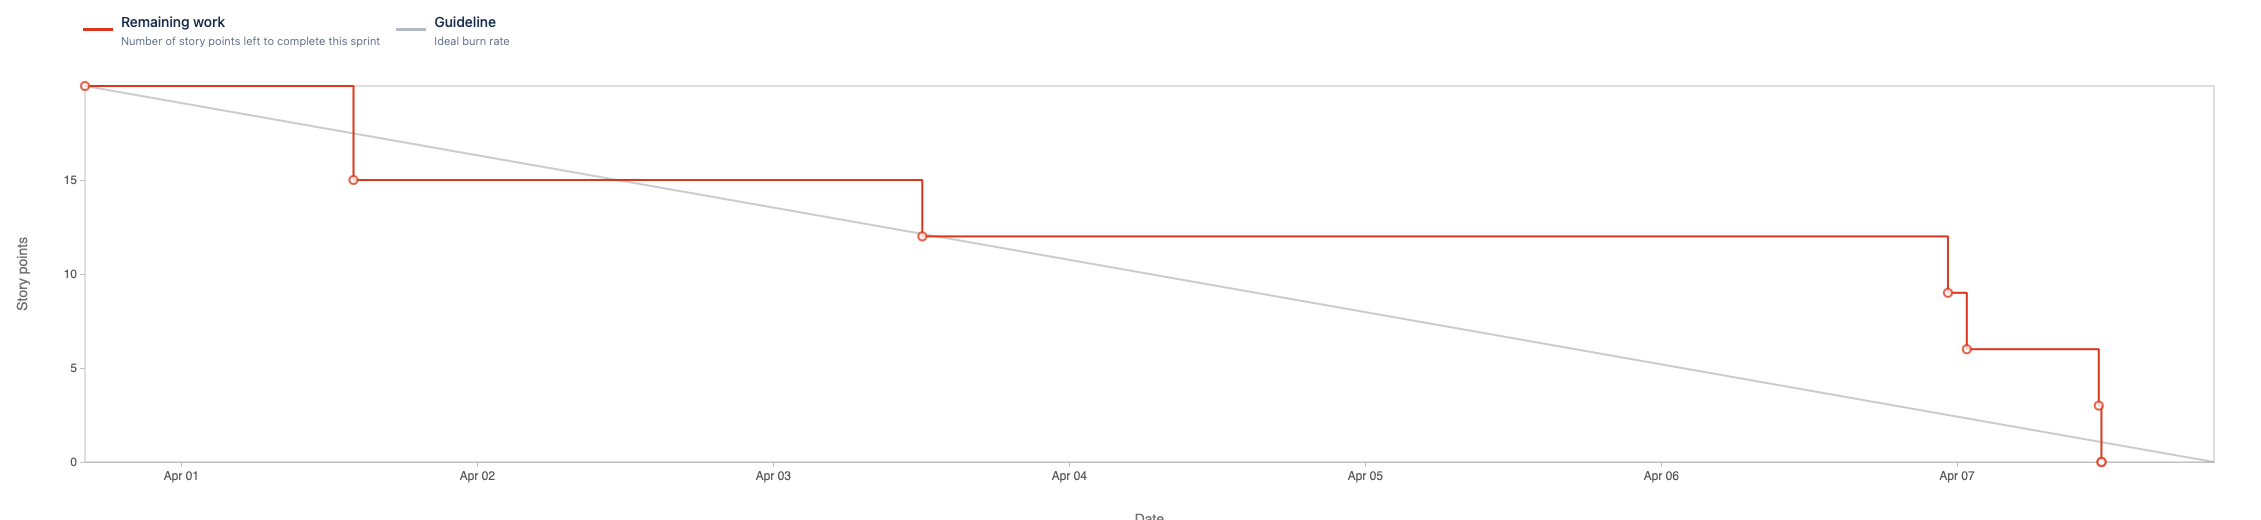
\includegraphics[width=1.0\textwidth]{img/sprint/sprint9.png}
    \caption{Sprint 9} \label{Img:Sprint+9}
\end{figure}

\subsection{Sprint 10 (09/04/23 - 23/04/23)}\label{sprint-0-090423---230422}
En este sprint se trabajó en el desarrollo de preguntas y respuestas, manejo de roles, perfil y actualización de usuario.\\
Favor apreciar el gráfico de burndown chart referente a ejecución de las tareas en este sprint, (ver figura~\ref{Img:Sprint+10}).
\begin{figure}[h]
    \centering
    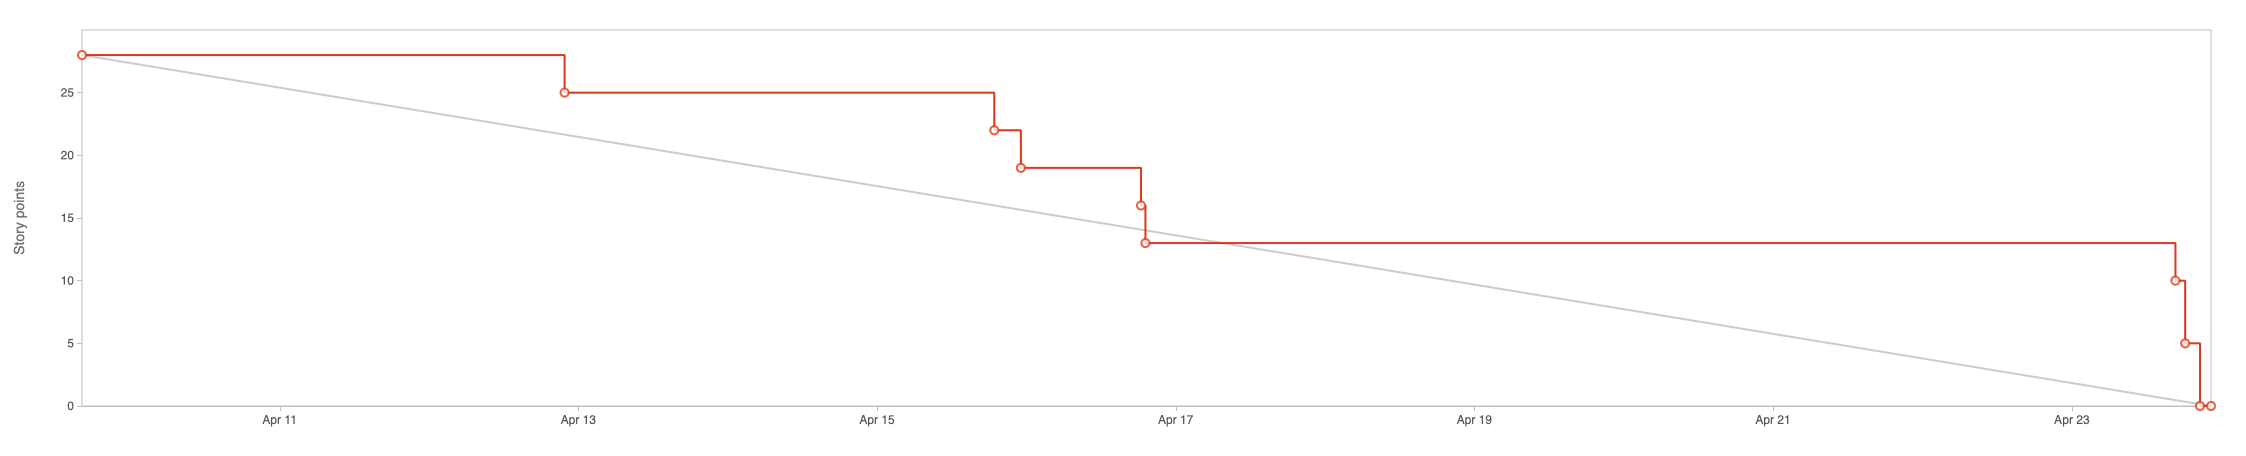
\includegraphics[width=1.0\textwidth]{img/sprint/sprint10.png}
    \caption{Sprint 10} \label{Img:Sprint+10}
\end{figure} 

\subsection{Sprint 11 (25/04/23 - 08/05/23)}\label{sprint-0-250423---080523}
En este sprint se trabajó con la eliminación de recetas y la actualización de las mismas, esto insumió trabajo debido a la eliminación de archivos adjuntos como por ejemplo imágenes.\\
Favor apreciar el gráfico de burndown chart referente a ejecución de las tareas en este sprint, (ver figura~\ref{Img:Sprint+11}).
\begin{figure}[h]
    \centering
    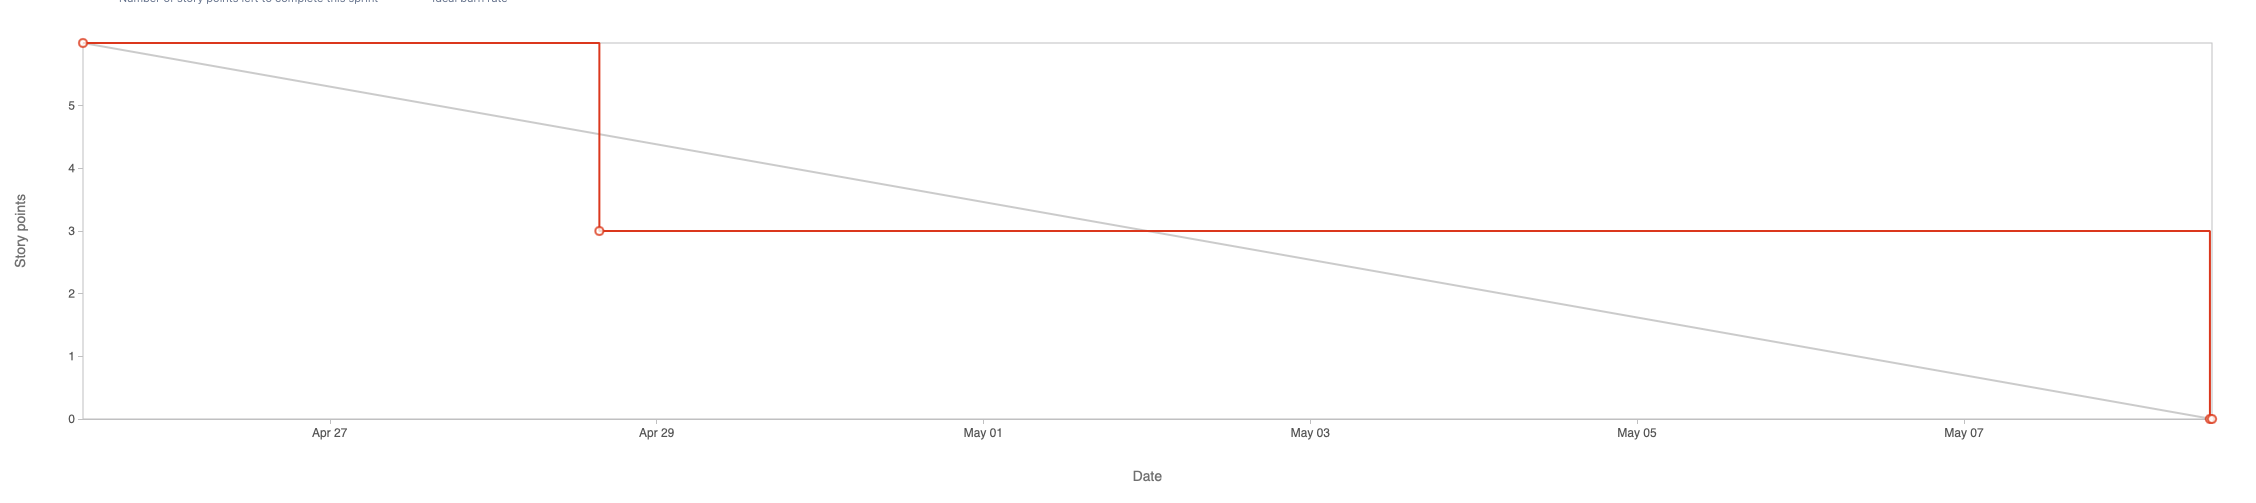
\includegraphics[width=1.0\textwidth]{img/sprint/sprint11.png}
    \caption{Sprint 11} \label{Img:Sprint+11}
\end{figure} 

\subsection{Sprint 12 (08/05/23 - 12/06/23)}\label{sprint-0-250423---080523}
En este sprint el alcance fue mayor, comprendiendo el desarrollo de muchas funcionalidades importantes, como la ficha de seguimiento del paciente, recordatorios, listado de médicos, mapas e interacción con la API externa para procesar datos del clima. \\
Favor apreciar el gráfico de burndown chart referente a ejecución de las tareas en este sprint, (ver figura~\ref{Img:Sprint+12}).
\begin{figure}[h]
    \centering
    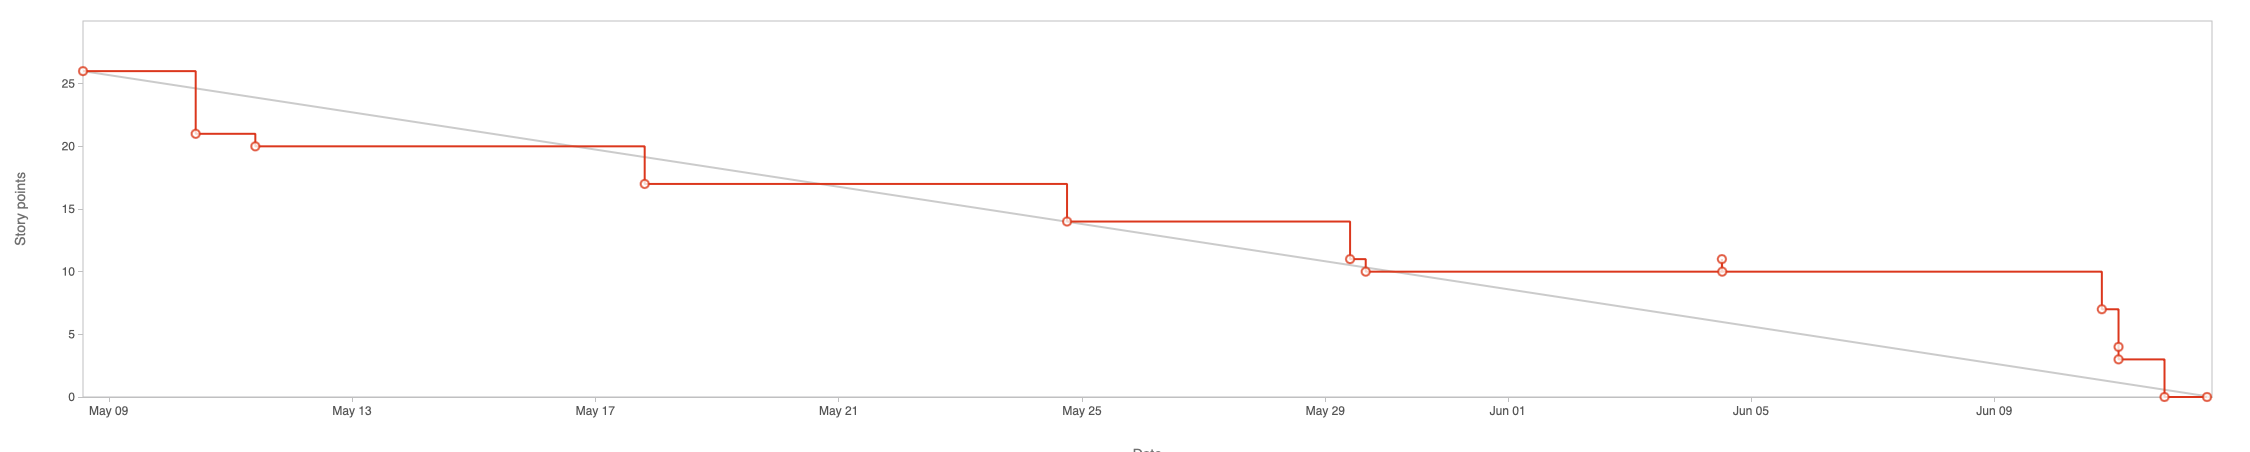
\includegraphics[width=1.0\textwidth]{img/sprint/sprint12.png}
    \caption{Sprint 12} \label{Img:Sprint+12}
\end{figure} 
\newpage
\subsection{Sprint 13 (12/06/23 - 18/06/23)}\label{sprint-0-120623---180623}
Durante este sprint se creó el chatbot que implicó un reto técnico así como en cuanto a conocimiento. Para ello, fue necesario crear el repositorio, el script para extraer información de una herramienta de EMUR (\href{https://brujulaem.uy/sitio/}{Brujula EM}), llevar a cabo la creación del motor de procesamiento, generar los vectores con FAISS para busqueda de cercanías y crear la API para el uso del chatbot.\\
Favor apreciar el gráfico de burndown chart referente a ejecución de las tareas en este sprint, (ver figura~\ref{Img:Sprint+13}).
\begin{figure}[h]
    \centering
    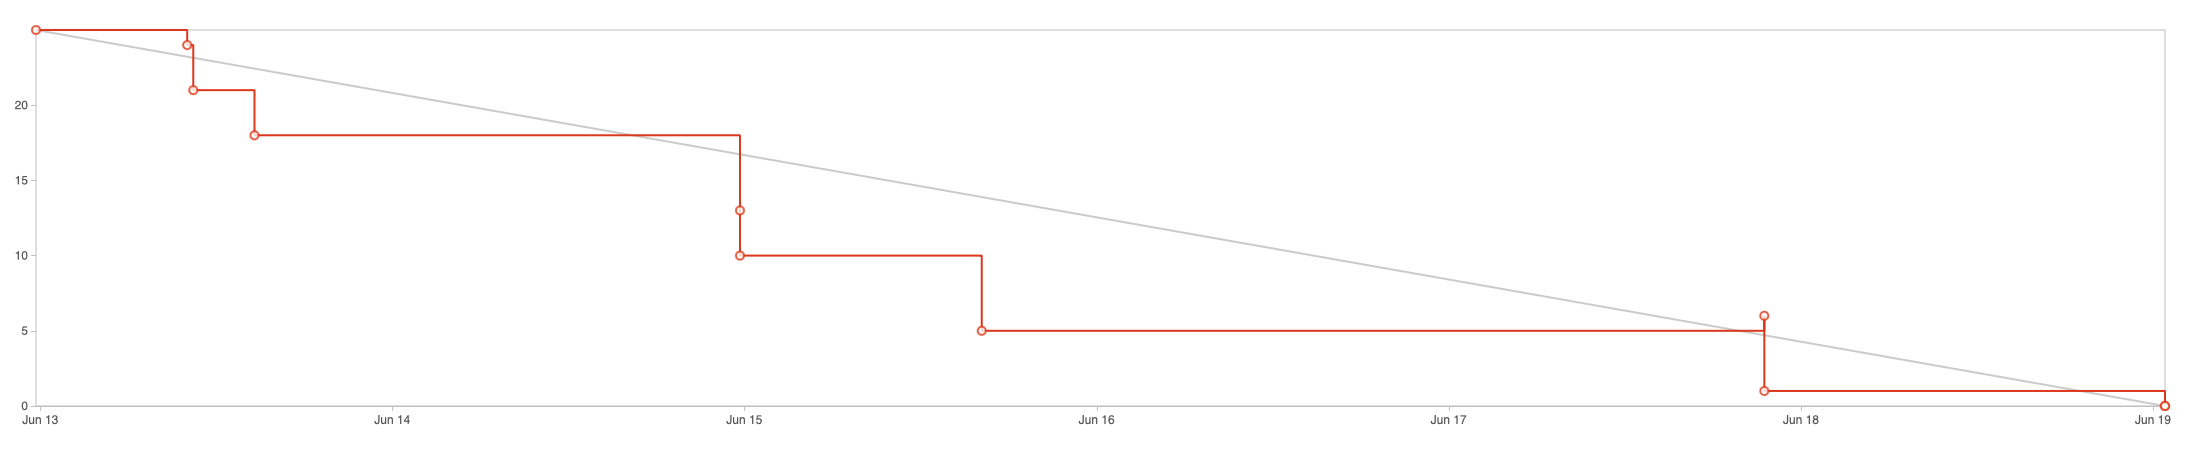
\includegraphics[width=1.0\textwidth]{img/sprint/sprint13.png}
    \caption{Sprint 13} \label{Img:Sprint+13}
\end{figure} 

\subsection{Sprint 14 (22/06/23 - 29/06/23)}\label{sprint-0-220623---290623}
Se generó todo los correspondiente a la documentación de los endpoints utilizando Swagger así como también se hizo el deploy a producción de los microservicios. Es de notar que en este sprint la ejecución fue más rápida debido a conocimientos previamente adquiridos a nivel laboral. \\
Favor apreciar el gráfico de burndown chart referente a ejecución de las tareas en este sprint, (ver figura~\ref{Img:Sprint+14}).
\begin{figure}[h]
    \centering
    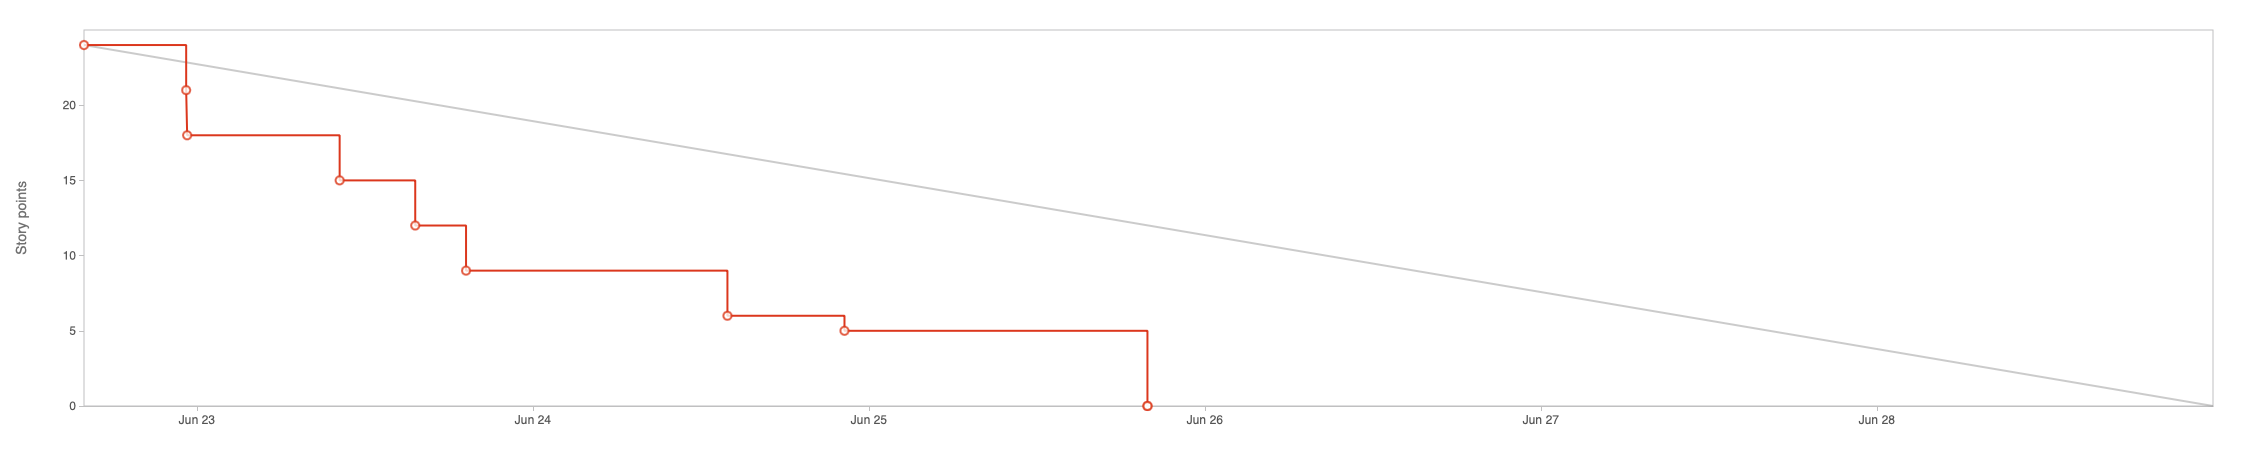
\includegraphics[width=1.0\textwidth]{img/sprint/sprint14.png}
    \caption{Sprint 14} \label{Img:Sprint+14}
\end{figure} 

\section{Estudio de viabilidad}
Un estudio de viabilidad es un análisis exhaustivo, desde diferentes perspectivas, que se realiza para determinar si un proyecto es factible y viable, o no. Este estudio facilita la toma de decisiones y permite identificar las fortalezas, debilidades, oportunidades y amenazas del proyecto.

\subsection{Viabilidad económica}
Un los aspectos clave dentro del estudio de viabilidad, es el económico, puesto que abarca el análisis de los costos en lo que se incurriría de implementarse el proyecto, en contraste con los posibles beneficios que se obtendrán tras su culminación. Así, a continuación, se muestran y analizan los costos y beneficios aproximados derivados del presente proyecto.

\subsubsection{Costes}
La estructura de costes del presente proyecto puede desglosarse en cuatro partidas: costes de personal, costes de hardware, costes de software y costes varios.
\subsubsection{Costes de personal:}
En este caso, el proyecto fue desarrollado por un único participante, en un período aproximado de 600 horas, durante 5 meses, a razón de 4 horas diarias, es decir, media jornada laboral, lo que equivaldría a 2 meses y medio, a razón de 8 horas diarias (jornada completa), que se redondearían a 3 meses de trabajo. Se ha estimado un salario neto de 715,55 USD en base a lo que suele cobrar un desarrollador en Uruguay. Esto se refleja en la tabla~\ref{tab:CostePersonal}.

\begin{longtable}[c]{@{}lr@{}}
\toprule
\multicolumn{1}{c}{\textbf{Concepto}} & \multicolumn{1}{c}{\textbf{Coste}} \\* \midrule
\endfirsthead
%
\endhead
%
\bottomrule
\endfoot
%
\endlastfoot
%
Salario mensual bruto & 890 USD \\
Seguridad Social & 174.45 USD (19,60\%) \\
Salario mensual neto & 715.55 USD \\
\hline
\textbf{Total 3 meses} & \textbf{2.146,65 USD} \\* \bottomrule \\
\caption{Coste mensual del personal}
\label{tab:CostePersonal}
\end{longtable}


Los datos necesarios para realizar estos cálculos fueron extraídos del simulador del Banco de Previsión Social \cite{web:bps}, en donde se debe especificar el salario mensual bruto del profesional, para que luego la plataforma haga las deducciones correspondientes al seguro social.

\subsubsection{Costes de hardware:}
Por ser un proyecto de desarrollo de software, el hardware se limitó al uso de una computadora personal amortizada a 5 años. Ver tabla~\ref{tab:CostesHardware}.

\begin{longtable}[c]{@{}lrr@{}}
\toprule
\multicolumn{1}{c}{\textbf{Concepto}} & \multicolumn{1}{c}{\textbf{Coste}} & \multicolumn{1}{c}{\textbf{Coste amortizado}} \\* \midrule
\endfirsthead
%
\endhead
%
\bottomrule
\endfoot
%
\endlastfoot
%
Ordenador portátil & 1.500 USD & 25 USD \\
Total & & 25 USD \\
Total 3 meses & & 75 USD \\ \hline
\caption{Costes de hardware}
\label{tab:CostesHardware}
\end{longtable}

\subsubsection{Costes de software:}

En este apartado se muestran los costos referentes al pago de licencias de software para el desarrollo del backend. Es importante considerar que, a fin de minimizar los costes, se trabajó en su mayoría con softwares gratuitos. Asimismo, al trabajar con un computador MAC no fue necesario pagar la licencia de uso del sistema operativo, como sí ocurre con Windows. Ver tabla~\ref{tab:CostesSoftware}.
\newpage
\begin{longtable}[c]{@{}lr@{}}
\toprule
\multicolumn{1}{c}{\textbf{Concepto}} & \multicolumn{1}{c}{\textbf{Coste Mensual}} \\* \midrule
\endfirsthead
%
\endhead
%
\bottomrule
\endfoot
%
\endlastfoot
%
SonarCloud & 10 USD \\
Digital Ocean & 24 USD \\
Base de datos Digital Ocean & 15 USD \\
Total & 49 USD \\
Total 3 meses & 147 USD \\ \hline
\caption{Costes de Software}
\label{tab:CostesSoftware}
\end{longtable}

\subsubsection{Costes varios:}
Por su parte, en este sección se detallan los costes del proyecto que no refieren ni al personal, ni al hardware o software, pero que aún así fueron necesarios para el desarrollo del backend en cuestión. Ver tabla~\ref{tab:CostesVarios}.

\begin{longtable}[c]{@{}lr@{}}
\toprule
\multicolumn{1}{c}{\textbf{Concepto}} & \multicolumn{1}{c}{\textbf{Coste}} \\* \midrule
\endfirsthead
%
\endhead
%
\bottomrule
\endfoot
%
\endlastfoot
%
Internet (3 meses) & 208,26 USD \\
Servicio eléctrico (3 meses) & 295,80 USD \\
Total & 504,06 USD \\ \hline
\caption{Costes varios}
\label{tab:CostesVarios}
\end{longtable}

\subsubsection{Coste Total:}
Por último, sólo resta sumar los resultados de las partidas anteriores para obtener el coste total del proyecto, lo cual arroja la cifra de 2.725,71 USD. El desglose de esta operación puede verse en la siguiente tabla. Ver tabla~\ref{tab:CostesTotal}

\begin{longtable}[c]{@{}lr@{}}
\toprule
\multicolumn{1}{c}{\textbf{Concepto}} & \multicolumn{1}{c}{\textbf{Coste}} \\* \midrule
\endfirsthead
%
\endhead
%
\bottomrule
\endfoot
%
\endlastfoot
%
Personal & 2.146,65 USD \\
Hardware & 75,00 USD \\
Software & 147 USD \\
Varios & 504,06 USD \\
Total & 2.872,71 USD \\ \hline
\caption{Costes totales}
\label{tab:CostesTotal}
\end{longtable}
\newpage
\subsection{Beneficios}
En vista de que el backend se desarrolló para una fundación sin ánimos de lucro enfocada en ayudar a personas afectadas con la EM, no se preve que la futura aplicación vaya a monetizarse de alguna forma para obtener algún beneficio económico siendo entonces de uso libre y gratuito.

\subsection{Viabilidad legal}
A continuación, se presentan las licencias requeridas para el desarrollo del presente proyecto, tanto del propio backend, como de su documentación, imágenes y vídeos. En este sentido, una licencia “es la facultad o permiso atribuido a una persona para ejercer una actividad, o gozar de ciertas libertades o concesiones fuera de las ordinarias, por situaciones particulares”.\cite{art:licencias}

Existe compatibilidad parcial entre las licencias de software de código abierto, siendo ésta mayor en unos casos que en otros. A continuación, se detallan las licencias de los módulos de terceros utilizados a lo largo de todo el desarrollo:

\begin{itemize}
\tightlist
\item
\textbf{Licencia MIT:} Licencia de software libre con gran flexibilidad que permite utilizar, modificar y distribuir software, al igual que la Apache 2.0 y la BSD-3. La licencia MIT es una de las más permisivas que hay, lo que implica que acepta un amplio uso del software, no tiene restricciones para uso comercial o privado, y no ofrece protección contra el uso de patentes.\\

\item
\textbf{Licencia Apache 2.0:} En comparación con la MIT, esta añade protección expresa contra las patentes, con su cláusula patentabilidad, permitiendo el uso comercial y privado.\\
\item
\textbf{Licencia BSD-3:} Por su parte, la BSD-3 posee políticas similares a la licencia MIT, permite el uso comercial y privado y no posee restricciones para uso comercial y privado. No obstante, viene con un cláusula de responsabilidad limitada.\\
\end{itemize}

Luego del análisis de los diferentes tipos de licencias de los módulos utilizados (ver tabla~\ref{tab:backend-modulo} y tabla~\ref{tab:chatbot-modulo}), se llegó a la conclusión de que la licencia más adecuada para este caso es la ofrecida por \emph{Apache 2.0}, a razón de las siguientes características:

\begin{itemize}
\tightlist
\item
Protección contra patentes: Lo que garantiza que cualquier usuario pueda hacer uso del software por la cláusula de concesión de patentes que proporciona derechos sobre cualquier patente del contribuidor, siempre que sea necesaria para el uso del programa.\\
\item
Permisividad: Los usuarios pueden modificar y distribuir el software sin necesidad de cumplir con otros requisitos especiales.\\
\item
Exención de responsabilidad y garantía: Lo que libera a los desarrolladores de responsabilidades legales si llegasen a producirse fallos de software.\\
\item 
Compatibilidad con otras licencias: Los usuarios podrán combinar el software con programas que estén bajo otras licencias.\\
\item 
 Notificación de cambios: Asegura que los usuarios sean informados de todo cambio o alteración en el código fuente.\\
 \item 
 Proyectos corporativos: Es ideal para este tipo de desarrollos por su flexibilidad y facilidad para inclusión en proyectos comerciales.\\
\end{itemize}

\begin{table}[H]
\centering
\begin{tabular}{llll}
\toprule
Módulo                     & Versión       & Descripción        & Licencia                    \\
\midrule
\texttt{Health Check}       & master & Middleware chequeo de status & MIT               \\
\texttt{AWS SDK }       & v1.44.237 & SDK para subir archivos & Apache 2.0               \\
\texttt{Imaging }       & v1.6.2 & Procesamiento de imágenes & MIT               \\
\texttt{GIN }       & v1.9.0 & Framework GO para APIs & MIT               \\
\texttt{JWT }       & v3.2.2 & Módulo para autenticación & MIT               \\
\texttt{Google UUID}       & v1.3.0 & Generación de UUID:  & BSD-3              \\
\texttt{Viper }       & v1.15.0 & Variables de entorno & MIT   \\     
\texttt{Testify}       & v1.8.2 & Librería para testing unitario & MIT   \\    
\texttt{Crypto}       & v0.10.0 & Biblioteca para criptografía   & BSD-3  \\    
\texttt{Text}       & v0.10.0 & Procesamiento de texto  & BSD-3  \\    
\texttt{Postgres}       & v1.5.0 & Librería para base de datos  & MIT  \\  
\texttt{Gorm}       & v1.24.7 & ORM para Golang  & MIT  \\  
\bottomrule
\end{tabular}
\caption{Licencias de módulos utilizados en el backend}
\label{tab:backend-modulo}
\end{table}


\begin{table}[H]
\centering
\begin{tabular}{llll}
\toprule
Módulo                     & Versión       & Descripción        & Licencia                    \\
\midrule
\texttt{Bs4}       & 4.12.2 & Librería para scrapping & MIT               \\
\texttt{Request}       & v2.31.0 & Librería para solicitudes HTTP & Apache 2.0               \\
\texttt{Urllib3}       & v2.0.3 & Cliente HTTP para Python & MIT               \\
\texttt{Alembic}       & v1.11.1 & Librería para migraciones & MIT               \\
\texttt{Dotenv}       & v1.0.0 & Variables de entorno & BSD-3               \\
\texttt{Psycopg2}       & v2.9.6 & Librería para base de datos & LGPL               \\
\texttt{Flask}       & v2.3.2 & Framework Python para APIs & BSD-3               \\
\texttt{Flasgger}       & v0.9.7b2 & Documentación Swagger & MIT               \\
\texttt{Gunicorn}       & v20.1.0 & Servidor Python & MIT               \\
\texttt{Langchain}       & v0.0.210 & Construcción de LLM & BSD-3               \\
\texttt{Gevent}       & v22.10.2 & Librería para corutinas & BSD-3               \\
\texttt{OpenAI}       & v0.27.8 & Librería para API OPENAI & BSD-3               \\
\texttt{Faiss}       & v1.7.4 & Similitud y agrupamiento de vectores & BSD-3               \\
\bottomrule
\end{tabular}
\caption{Licencias de módulos utilizados en el chatbot}
\label{tab:chatbot-modulo}
\end{table}